\chapter{Specifikacija programske potpore}

\section{Funkcionalni zahtjevi}

\textbf{\textit{dio 1. revizije}}\\

\textit{Navesti \textbf{dionike} koji imaju \textbf{interes u ovom sustavu} ili  \textbf{su nositelji odgovornosti}. To su prije svega korisnici, ali i administratori sustava, naručitelji, razvojni tim.}\\

\textit{Navesti \textbf{aktore} koji izravno \textbf{koriste} ili \textbf{komuniciraju sa sustavom}. Oni mogu imati inicijatorsku ulogu, tj. započinju određene procese u sustavu ili samo sudioničku ulogu, tj. obavljaju određeni posao. Za svakog aktora navesti funkcionalne zahtjeve koji se na njega odnose.}\\


\noindent \textbf{Dionici:}

\begin{packed_enum}
	
	\item Studentski centar Sveučilišta u Zagrebu (naručitelj)
	\item Korisnici praonice veša				
	\item Zaposlenici praonice veša
	\item Administrator sustava
	\item Razvojni tim
	
\end{packed_enum}

\noindent \textbf{Aktori i njihovi funkcionalni zahtjevi:}


\begin{packed_enum}
	\item  \underbar{Neregistrirani/neprijavljeni korisnik (inicijator) može:}
	
	\begin{packed_enum}
		
		\item napraviti novi korisnički račun za koji su mu potrebni adresa e-pošte, lozinka, ime, prezime, JMBAG i broj mobitela
		\item vidjeti oglase za posao (osobe koje ne žive u domu i nisu studenti, odnosno nemaju pravo koristiti praonicu, mogu se zaposliti u praonici, prijave za oglas ne idu putem aplikacije, već še molba i životopis šalju na adresu e-pošte navedenu u oglasu)
		\item vidjeti podatke o praonici 
		
		\begin{packed_enum}
			\item radno vrijeme praonice
			\item cijene pranja i sušenja
		\end{packed_enum}
		
	\end{packed_enum}
	
	\item  \underbar{Registrirani korisnik (inicijator) može:}
	
	\begin{packed_enum}
		
		\item sve akcije navedene za neregistriranog korisnika
		\item prijaviti se u sustav
		\item pristupiti kalendaru u kojem se prikazuju slobodni i popunjeni termini
		\item rezervirati termin za pranje i sušenje veša
		\item prilikom rezervacije odabrati način plaćanja (putem aplikacije ili na blagajni doma)
		\item postaviti bilješku na rezervaciju
		\item urediti ili otkazati rezervirani termin (do 24 sata prije termina)
		\item ocijeniti radnika u praonici koji je bio u njihovom terminu pranja
		\item pristupiti zidu s obavijestima o izgubljenim stvarima
		\item pregled vlastitog profila i uređivanje podataka
		
	\end{packed_enum}
	
	\item  \underbar{Zaposlenik (inicijator) može:}
	
	\begin{packed_enum}
		
		\item prijaviti se u sustav
		\item pregled vlastitog profila i uređivanje podataka
		\item pristupiti zidu s obavijestima o izgubljenim stvarima
		\item promijeniti vrijeme pauze
		\item označiti tko je posudio košaru za rublje
		\item poslati obavijest na mail osobi kojoj je gotovo rublje
		\item označiti da se netko nije pojavio u terminu i osloboditi ga
		\item objaviti fotografiju izgubljenog (zaboravljenog) odjevnog predmeta u praonici
		\item pregledati termine za radni dan
		\item potvrditi registraciju korisnika
		
	\end{packed_enum}
	
	\item  \underbar{Administrator (inicijator) može:}
	
	\begin{packed_enum}
		
		\item sve akcije navedene za zaposlenika
		\item objaviti, urediti i obrisati oglas za posao
		\item promijeniti radno vrijeme praonice
		\item obaviti promjenu cijene pranja
		\item obaviti promjenu cijene sušenja
		\item blokirati pristup aplikaciji bilo kojem korisniku
		\item dodavanje, brisanje i uređivanje zaposlenika i korisnika
		\item pregled recenzija svih zaposlenika
		
	\end{packed_enum}
	
	\item  \underbar{Baza podataka (sudionik) može:}
	
	\begin{packed_enum}
		
		\item spigl 
		\item funkcionalnost 2
		
	\end{packed_enum}
	
\end{packed_enum}

\eject 



\subsection{Obrasci uporabe}

\textbf{\textit{dio 1. revizije}}

\subsubsection{Opis obrazaca uporabe}
\textit{Funkcionalne zahtjeve razraditi u obliku obrazaca uporabe. Svaki obrazac je potrebno razraditi prema donjem predlošku. Ukoliko u nekom koraku može doći do odstupanja, potrebno je to odstupanje opisati i po mogućnosti ponuditi rješenje kojim bi se tijek obrasca vratio na osnovni tijek.}\\


\noindent \underbar{\textbf{UC$<$broj obrasca$>$ -$<$ime obrasca$>$}}
\begin{packed_item}
	
	\item \textbf{Glavni sudionik: }$<$sudionik$>$
	\item  \textbf{Cilj:} $<$cilj$>$
	\item  \textbf{Sudionici:} $<$sudionici$>$
	\item  \textbf{Preduvjet:} $<$preduvjet$>$
	\item  \textbf{Opis osnovnog tijeka:}
	
	\item[] \begin{packed_enum}
		
		\item $<$opis korak jedan$>$
		\item $<$opis korak dva$>$
		\item $<$opis korak tri$>$
		\item $<$opis korak četiri$>$
		\item $<$opis korak pet$>$
	\end{packed_enum}
	
	\item  \textbf{Opis mogućih odstupanja:}
	
	\item[] \begin{packed_item}
		
		\item[2.a] $<$opis mogućeg scenarija odstupanja u koraku 2$>$
		\item[] \begin{packed_enum}
			
			\item $<$opis rješenja mogućeg scenarija korak 1$>$
			\item $<$opis rješenja mogućeg scenarija korak 2$>$
			
		\end{packed_enum}
		\item[2.b] $<$opis mogućeg scenarija odstupanja u koraku 2$>$
		\item[3.a] $<$opis mogućeg scenarija odstupanja  u koraku 3$>$
		
	\end{packed_item}
\end{packed_item}

\noindent \underbar{\textbf{UC1 - Registracija}}
\begin{packed_item}
	
	\item \textbf{Glavni sudionik: } Neregistrirani korisnik
	\item  \textbf{Cilj:} Stvoriti korisnički račun za pristup sustavu
	\item  \textbf{Sudionici:}  Baza podataka + pitanje (ako radnik treba potvrditi, je li i on sudionik?)
	\item  \textbf{Preduvjet:} -
	\item  \textbf{Opis osnovnog tijeka:}
	
	\item[] \begin{packed_enum}
		
		\item Korisnik odabire opciju za registraciju
		\item Korisnik unosi potrebne korisničke podatke
		\item Korisnik dobiva obavijest o slanju registracije na potvrdu
		\item Korisnik odlazi osobno u praonicu s potvrdom da stanuje u domu 
		\item Radnik u praonici potvrđuje prijavu nakon uvjeravanja da osoba stanuje u domu
		\item Korisnik prima obavijest o uspješnoj registraciji
	\end{packed_enum}
	
	\item  \textbf{Opis mogućih odstupanja:}
	
	\item[] \begin{packed_item}
		
		\item[2.a] Odabir već zauzete ili nepostojeće adrese e-pošte te neispravno popunjavanje obrasca
		\item[] \begin{packed_enum}
			
			\item Sustav obavještava korisnika o neuspjeloj registraciji i vraća ga na natrag stranicu za registraciju korisnika
			\item Korisnik mijenja potrebne podatke te se ponovno pokušava registrirati ili odustaje od registracije
			
		\end{packed_enum}
		
		\item[4.a] Korisnik zaboravi odnijeti potvrdu o stanovanju u studentskom domu u praonicu
		\item[] \begin{packed_enum}
			
			\item Sustav obavještava korisnika da odnese potvrdu u praonicu
			\item Nakon određenog vremena pokušaj registracije briše se iz sustava
			
		\end{packed_enum}
		
		\item[5.a] Radnik u praonici nije potvrdio registraciju korisnika
		\item[] \begin{packed_enum}
			
			\item Korisnik ponovno odlazi u praonicu s potvrdom
			
		\end{packed_enum}
		
		\item[5.a] Radnik u praonici potvrdio je ili odbio zahtjev za registracijom krivog korisnika
		\item[] \begin{packed_enum}
			
			\item Radnik obavještava administratora o tome kojeg je korisnika zabunom potvrdio ili odbio, te administrator promijeni podatke u bazi podataka
			
		\end{packed_enum}
		
		
	\end{packed_item}	
\end{packed_item}

\noindent \underbar{\textbf{UC2 - Prijava}}
\begin{packed_item}
	
	\item \textbf{Glavni sudionik: } Registrirani korisnik,  Zaposlenik, Administrator
	\item  \textbf{Cilj:} Prijava za pristup sustavu
	\item  \textbf{Sudionici:} Baza podataka
	\item  \textbf{Preduvjet:} Korisnik je registriran u sustavu
	\item  \textbf{Opis osnovnog tijeka:}
	
	\item[] \begin{packed_enum}
		
		\item Korisnik ispunjava potrebne podatke za prijavu (e-mail i lozinku)
		\item Korisniku se omogućava pristup značajkama specifičnim za njegovu razinu pristupa

	\end{packed_enum}
	
	\item  \textbf{Opis mogućih odstupanja:}
	
	\item[] \begin{packed_item}
		
		\item[2.a] Unos krive kombinacije e-mail-a i lozinke
		\item[] \begin{packed_enum}
			
			\item Sustav korisnika vraća na početnu stranicu i dojavljuje da je prijava neuspjela
			\item Korisnik ponovno upisuje podatke ili odustaje od prijave
			
		\end{packed_enum}
	\end{packed_item}
\end{packed_item}

\noindent \underbar{\textbf{UC3 - Pregled vlastitog profila i uređivanje podataka}}
\begin{packed_item}
	
	\item \textbf{Glavni sudionik: } Registrirani korisnik, Zaposlenik, Administrator
	\item  \textbf{Cilj:} Omogućuje pregledavanje i modificiranje osobnih podataka
	\item  \textbf{Sudionici:} Baza podataka
	\item  \textbf{Preduvjet:} Korisnik je prijavljen u sustav
	\item  \textbf{Opis osnovnog tijeka:}
	
	\item[] \begin{packed_enum}
		
		\item Korisnik odabire opciju za prikaz vlastitog profila
		\item Korisniku se prikazuju njegovi osobni podaci
		\item Klikom na gumb za izmjenu korisniku se otvara obrazac za promjenu
		
	\end{packed_enum}
	
	\item  \textbf{Opis mogućih odstupanja:}
	
	\item[] \begin{packed_item}
		
		\item[2.a] Korisnik neispravno popunjava obrazac za promjenu
		\item[] \begin{packed_enum}
			
			\item Korisniku se ispisuje upozorenje
			\item Promjena ostaje nezabilježena u sustavu
			
		\end{packed_enum}
	\end{packed_item}
\end{packed_item}

\noindent \underbar{\textbf{UC4 - Rezervacija termina za pranje veša}}
\begin{packed_item}
	
	\item \textbf{Glavni sudionik: } Registrirani korisnik
	\item  \textbf{Cilj:} Rezerviranje željenog termina u praonici
	\item  \textbf{Sudionici:} Baza podataka
	\item  \textbf{Preduvjet:} Korisnik je prijavljen u sustav
	\item  \textbf{Opis osnovnog tijeka:}
	
	\item[] \begin{packed_enum}
		
		\item Korisnik odabire opciju za rezervaciju termina
		\item Korisniku se prikazuje kalendar sa slobodnim terminima
		\item Korisnik odabire slobodan termin
		\item Korisnik odabire način plaćanja
		\item Korisniku se nudi opcija stavljanja bilješke na rezervaciju
		\item Rezervacija se registrira u sustavu
		
	\end{packed_enum}
	
	\item  \textbf{Opis mogućih odstupanja:}
	
	\item[] \begin{packed_item}
		
		
		\item[2.a] Nema slobodnih termina
		\item[] \begin{packed_enum}
			
			\item Korisniku se ispisuje poruka da nema slobodnih termina
			
		\end{packed_enum}
		
	\end{packed_item}
\end{packed_item}

\noindent \underbar{\textbf{UC4.1 - Plaćanje rezervacije}}
\begin{packed_item}
	
	\item \textbf{Glavni sudionik: } Registrirani korisnik
	\item  \textbf{Cilj:} Plaćanje pranja ili sušenja
	\item  \textbf{Sudionici:} Baza podataka
	\item  \textbf{Preduvjet:} Korisnik je prijavljen u sustav
	\item  \textbf{Opis osnovnog tijeka:}
	
	\item[] \begin{packed_enum}
		
		\item Korisnik odabire opciju plaćanja
		\item Izvršava se plaćanje u sustavu ili na blagajni
		
	\end{packed_enum}
	
	\item  \textbf{Opis mogućih odstupanja:}
	
	\item[] \begin{packed_item}
		
		\item[2.a] Korisnik nema sredstava
		\item[] \begin{packed_enum}
			
			\item Korisniku se ispisuje upozorenje da nema sredstava
			\item Korisniku se nudi plaćanje na blagajni
			
		\end{packed_enum}
		
	\end{packed_item}
\end{packed_item}


\noindent \underbar{\textbf{UC5 - Pristup kalendaru sa terminima}}
\begin{packed_item}
	
	\item \textbf{Glavni sudionik: }Registrirani korisnik
	\item  \textbf{Cilj:} Pregledati slobodne termine
	\item  \textbf{Sudionici:} Baza podataka
	\item  \textbf{Preduvjet:} Korisnik je prijavljen u sustav
	\item  \textbf{Opis osnovnog tijeka:}
	
	\item[] \begin{packed_enum}
		
		\item Korisnik odabire opciju za prikaz kalendara
		\item Korisniku se prikazuje kalendar sa terminima

	\end{packed_enum}
	
\end{packed_item}

\noindent \underbar{\textbf{UC6 - Uređivanje rezerviranog termina}}
\begin{packed_item}
	
	\item \textbf{Glavni sudionik: } Registrirani korisnik
	\item  \textbf{Cilj:} Urediti postojeću rezervaciju termina
	\item  \textbf{Sudionici:} Baza podataka
	\item  \textbf{Preduvjet:} Korisnik je prijavljen u sustav i ima rezervirani termin
	\item  \textbf{Opis osnovnog tijeka:}
	
	\item[] \begin{packed_enum}
		
		\item Korisnik u kalendaru odabire rezervirani termin
		\item Korisniku se nudi izbor pomicanja ili otkazivanja termina te opcija dodavanja bilješke
		\item Korisnik odabire željenu akciju
	\end{packed_enum}
	
	\item  \textbf{Opis mogućih odstupanja:}
	
	\item[] \begin{packed_item}
		
		\item[2.a] Preostalo je manje od 24 sata do termina, a korisnik želi preseliti/otkazati termin
		\item[] \begin{packed_enum}
			
			\item Korisniku se pojavljuje poruka kako je termin nemoguće preseliti/otkazati termin
			\item Korisnika se vraća na kalendar
			
		\end{packed_enum}
		
	\end{packed_item}
\end{packed_item}

\noindent \underbar{\textbf{UC7 - Ocjenjivanje radnika u terminu}}
\begin{packed_item}
	
	\item \textbf{Glavni sudionik: }Registrirani korisnik
	\item  \textbf{Cilj:} Ocijeniti radnika u terminu korištenja praonice
	\item  \textbf{Sudionici:} Baza podataka
	\item  \textbf{Preduvjet:} Korisnik je prijavljen u sustav
	\item  \textbf{Opis osnovnog tijeka:}
	
	\item[] \begin{packed_enum}
		
		\item Korisniku se nakon termina pranja nudi opcija ocjenjivanja
		\item Korisnik unosi ocjenu
		\item Ocjena se bilježi u sustavu
	\end{packed_enum}
		
\end{packed_item}

\noindent \underbar{\textbf{UC8 - Pregled zida s obavijestima o izgubljenim stvarima}}
\begin{packed_item}
	
	\item \textbf{Glavni sudionik: } Registrirani korisnik, Zaposlenik, Administrator 
	\item  \textbf{Cilj:} Pristup zidu s obavijestima o izgubljenim stvarima
	\item  \textbf{Sudionici:} Baza podataka
	\item  \textbf{Preduvjet:} Korisnik je prijavljen u sustav
	\item  \textbf{Opis osnovnog tijeka:}
	
	\item[] \begin{packed_enum}
		
		\item Korisnik odabire opciju zida s obavijestima o izgubljenim stvarima
		\item Korisniku se prikazuje zid s obavijestima o izgubljenim stvarima
	\end{packed_enum}
\end{packed_item}

\noindent \underbar{\textbf{UC9 - Pregled podataka o praonici}}
\begin{packed_item}
	
	\item \textbf{Glavni sudionik: } Registrirani korisnik, neregistrirani korisnik
	\item  \textbf{Cilj:} Prikaz podataka o praonici
	\item  \textbf{Sudionici:} Baza podataka
	\item  \textbf{Preduvjet:} -
	\item  \textbf{Opis osnovnog tijeka:}
	
	\item[] \begin{packed_enum}
		
		\item Korisnik odabire opciju za prikaz podataka o praonici
		\item Korisniku se prikazuju podaci o praonici
		
	\end{packed_enum}
	
\end{packed_item}

\noindent \underbar{\textbf{UC10 - Pregled oglasa za posao}}
\begin{packed_item}
	
	\item \textbf{Glavni sudionik:} Registrirani korisnik, neregistrirani korisnik
	\item  \textbf{Cilj:} Prikaz oglasa za posao
	\item  \textbf{Sudionici:} Baza podataka
	\item  \textbf{Preduvjet:} -
	\item  \textbf{Opis osnovnog tijeka:}
	
	\item[] \begin{packed_enum}
		
		\item Korisnik odabire opciju za prikaz oglasa za posao
		\item Korisniku se prikazuju oglasi
		
	\end{packed_enum}
	
\end{packed_item}

\noindent \underbar{\textbf{UC11 - Objava oglasa za posao}}
\begin{packed_item}
	
	\item \textbf{Glavni sudionik: } Administrator
	\item  \textbf{Cilj:} Objaviti oglas za studentski posao
	\item  \textbf{Sudionici:} Baza podataka
	\item  \textbf{Preduvjet:} Postoji otvorena pozicija u praonici i korisnik je registriran i dodijeljena su mu prava administratora
	\item  \textbf{Opis osnovnog tijeka:}
	
	\item[] \begin{packed_enum}
		
		\item Administrator odabire opciju za stvaranje novog oglasa
		\item Administrator ispunjava tekst i podatke oglasa
		\item Oglas se objavljuje odabirom opcije za objavljivanje oglasa.
	\end{packed_enum}
	
	\item  \textbf{Opis mogućih odstupanja:}
	
	\item[] \begin{packed_item}
		
		\item[2.a] Pogrešno uneseni podaci o natječaju
		\item[] \begin{packed_enum}
			
			\item Omogućiti editiranje oglasa nakon objave
			
		\end{packed_enum}				
	\end{packed_item}
\end{packed_item}

\noindent \underbar{\textbf{UC12 - Promjena radnog vremena}}
\begin{packed_item}
	
	\item \textbf{Glavni sudionik: } Administrator
	\item  \textbf{Cilj:} Promijeniti radno vrijeme praonice
	\item  \textbf{Sudionici:} Baza podataka
	\item  \textbf{Preduvjet:} Korisnik je registriran i dodijeljena su mu prava administratora
	\item  \textbf{Opis osnovnog tijeka:}
	
	\item[] \begin{packed_enum}
		
		\item Administrator odabire opciju promjene radnog vremena
		\item Prikaže se modal za odabir novog radnog vremena
		\item Administrator unosi novo radno vrijeme
		\item Administrator odabire opciju za potvrdu novog radnog vremena
	\end{packed_enum}
\end{packed_item}

\noindent \underbar{\textbf{UC - Promjena cijene pranja}}
\begin{packed_item}
	
	\item \textbf{Glavni sudionik: } Administrator
	\item  \textbf{Cilj:} Promijeniti cijenu jednog pranja
	\item  \textbf{Sudionici:} Baza podataka
	\item  \textbf{Preduvjet:} Korisnik je registriran i dodijeljena su mu prava administratora
	\item  \textbf{Opis osnovnog tijeka:}
	
	\item[] \begin{packed_enum}
		
		\item Administrator odabire opciju promjene cijene pranja
		\item Prikaže se modal za unos nove cijene pranja
		\item Administrator unosi novu cijenu pranja
		\item Administrator odabire opciju za potvrdu nove cijene pranja
	\end{packed_enum}
\end{packed_item}

\noindent \underbar{\textbf{UC14 - Promjena cijene sušenja}}
\begin{packed_item}
	
	\item \textbf{Glavni sudionik: } Administrator
	\item  \textbf{Cilj:} Promijeniti cijenu jednog sušenja
	\item  \textbf{Sudionici:} Baza podataka
	\item  \textbf{Preduvjet:} Korisnik je registriran i dodijeljena su mu prava administratora
	\item  \textbf{Opis osnovnog tijeka:}
	
	\item[] \begin{packed_enum}
		
		\item Administrator odabire opciju promjene cijene sušenja
		\item Prikaže se modal za unos nove cijene sušenja
		\item Administrator unosi novu cijenu sušenja
		\item Administrator odabire opciju za potvrdu nove cijene sušenja
	\end{packed_enum}
\end{packed_item}

\noindent \underbar{\textbf{UC15 - Zabrana pristupa korisniku}}
\begin{packed_item}
	
	\item \textbf{Glavni sudionik: } Administrator
	\item  \textbf{Cilj:} Zabraniti pristup uslugama praonice korisniku
	\item  \textbf{Sudionici:} Baza podataka
	\item  \textbf{Preduvjet:} Korisnik je registriran i dodijeljena su mu prava administratora
	\item  \textbf{Opis osnovnog tijeka:}
	
	\item[] \begin{packed_enum}
		
		\item Administrator odabire opciju zabrane pristupa korisnicima
		\item Prikaže se lista svih ispravno registriranih korisnika
		\item Administrator odabire korisnika ili više njih
		\item Administrator odabire opciju za potvrdu zabrane pristupa
	\end{packed_enum}
\end{packed_item}

\noindent \underbar{\textbf{UC16 - Uređivanje oglasa za posao}}
\begin{packed_item}
	
	\item \textbf{Glavni sudionik: } Administrator
	\item  \textbf{Cilj:} Promijeniti podatke unesene u oglasu za posao
	\item  \textbf{Sudionici:} Baza podataka
	\item  \textbf{Preduvjet:} Korisnik je registriran i dodijeljena su mu prava administratora, te postoje objavljeni oglasi
	\item  \textbf{Opis osnovnog tijeka:}
	
	\item[] \begin{packed_enum}
		
		\item Administrator odabire opciju pregleda oglasa
		\item Prikaže se lista svih objavljenih oglasa
		\item Administrator odabire oglas koji želi urediti
		\item Administrator unosi izmjene
		\item Administrator odabire opciju za potvrdu izmjena
	\end{packed_enum}
\end{packed_item}

\noindent \underbar{\textbf{UC17 - Brisanje oglasa za posao}}
\begin{packed_item}
	
	\item \textbf{Glavni sudionik: } Administrator
	\item  \textbf{Cilj:} Obrisati oglas za posao
	\item  \textbf{Sudionici:} Baza podataka
	\item  \textbf{Preduvjet:} Korisnik je registriran i dodijeljena su mu prava administratora, te postoje objavljeni oglasi
	\item  \textbf{Opis osnovnog tijeka:}
	
	\item[] \begin{packed_enum}
		
		\item Administrator odabire opciju pregleda oglasa
		\item Prikaže se lista svih objavljenih oglasa
		\item Administrator odabire oglas koji želi obrisati
		\item Administrator odabire opciju za brisanje
		\item Administrator odabire opciju za potvrdu izmjena
	\end{packed_enum}
\end{packed_item}

\noindent \underbar{\textbf{UC18 - Dodavanje novih korisnika}}
\begin{packed_item}
	
	\item \textbf{Glavni sudionik: } Administrator
	\item  \textbf{Cilj:} Dodati novog korisnika
	\item  \textbf{Sudionici:} Baza podataka
	\item  \textbf{Preduvjet:} Korisnik je registriran i dodijeljena su mu prava administratora
	\item  \textbf{Opis osnovnog tijeka:}
	
	\item[] \begin{packed_enum}
		
		\item Administrator odabire opciju pregleda korisnika
		\item Prikaže se lista svih registriranih korisnika i zaposlenika
		\item Administrator odabire opciju za stvaranje novog korisnika
		\item Administrator unosi podatke o novom korisniku
		\item Administrator odabire opciju za potvrdu izmjena
	\end{packed_enum}
\end{packed_item}

\noindent \underbar{\textbf{UC19 - Brisanje korisnika}}
\begin{packed_item}
	
	\item \textbf{Glavni sudionik: } Administrator
	\item  \textbf{Cilj:} Obrisati korisnika
	\item  \textbf{Sudionici:} Baza podataka
	\item  \textbf{Preduvjet:} Korisnik je registriran i dodijeljena su mu prava administratora, te postoje registrirani korisnici
	\item  \textbf{Opis osnovnog tijeka:}
	
	\item[] \begin{packed_enum}
		
		\item Administrator odabire opciju pregleda korisnika
		\item Prikaže se lista svih registriranih korisnika i zaposlenika
		\item Administrator odabire korisnika kojeg želi obrisati
		\item Administrator odabire opciju za brisanje korisnika
		\item Administrator odabire opciju za potvrdu izmjena
	\end{packed_enum}
\end{packed_item}

\noindent \underbar{\textbf{UC20 - Uređivanje korisnika}}
\begin{packed_item}
	
	\item \textbf{Glavni sudionik: } Administrator
	\item  \textbf{Cilj:} Urediti podatke o korisniku
	\item  \textbf{Sudionici:} Baza podataka
	\item  \textbf{Preduvjet:} Korisnik je registriran i dodijeljena su mu prava administratora, te postoje registrirani korisnici
	\item  \textbf{Opis osnovnog tijeka:}
	
	\item[] \begin{packed_enum}
		
		\item Administrator odabire opciju pregleda korisnika
		\item Prikaže se lista svih registriranih korisnika i zaposlenika
		\item Administrator odabire korisnika čije podatke želi urediti
		\item Administrator unosi izmjene
		\item Administrator odabire opciju za potvrdu izmjena
	\end{packed_enum}
\end{packed_item}

\noindent \underbar{\textbf{UC21 - Pregled recenzija svih zaposlenika}}
\begin{packed_item}
	
	\item \textbf{Glavni sudionik: } Administrator
	\item  \textbf{Cilj:} Pregled recenzije zaposlenika
	\item  \textbf{Sudionici:} Baza podataka
	\item  \textbf{Preduvjet:} Korisnik je registriran i dodijeljena su mu prava administratora, te postoje recenzije zaposlenika
	\item  \textbf{Opis osnovnog tijeka:}
	
	\item[] \begin{packed_enum}
		
		\item Administrator odabire opciju pregleda zaposlenika
		\item Prikaže se lista svih zaposlenika
		\item Administrator odabire zaposlenika čije recenzije želi pogledati
		\item Administrator odabire opciju za pregled recenzija
	\end{packed_enum}
\end{packed_item}

\noindent \underbar{\textbf{UC22 - Oznaka posudbe košare za rublje}}
\begin{packed_item}
	
	\item \textbf{Glavni sudionik: }Zaposlenik
	\item  \textbf{Cilj:} Označiti osobu koja je posudila košaru za rublje
	\item  \textbf{Sudionici:} Baza podataka
	\item  \textbf{Preduvjet:} -
	\item  \textbf{Opis osnovnog tijeka:}
	
	\item[] \begin{packed_enum}
		
		\item Zaposlenik odabire korisnika koji je posudio košaru
		\item Zaposlenik odabire opciju za posudbu  
		
	\end{packed_enum}
	
	\item  \textbf{Opis mogućih odstupanja:}
	
	\item[] \begin{packed_item}
		
		\item[2.a] Korisnik već ima posuđenu košaru 
		\item[] \begin{packed_enum}
			
			\item Onemogućuje mu se posudba nove košare dok ne vrati staru
			
		\end{packed_enum}
		\item[2.b] Korisnik ne vrati posuđenu košaru
		\item[] \begin{packed_enum}
			
			\item Korisnik dobiva opomenu
			
		\end{packed_enum}
		
		
	\end{packed_item}
\end{packed_item}
\noindent \underbar{\textbf{UC23 - Slanje obavijesti na mail}}
\begin{packed_item}
	
	\item \textbf{Glavni sudionik: }Zaposlenik, Administrator
	\item  \textbf{Cilj:} Obavijestiti korisnika kojem je rublje gotovo
	\item  \textbf{Sudionici:} Baza podataka
	\item  \textbf{Preduvjet:} -
	\item  \textbf{Opis osnovnog tijeka:}
	
	\item[] \begin{packed_enum}
		
		\item Zaposlenik odabire korisnika kojem je rublje gotovo
		\item Zaposlenik odabire njegovu mail adresu 
		\item Zaposlenik šalje obavijest
		\item Korisnik prima obavijest
		
	\end{packed_enum}
	
\end{packed_item}
\noindent \underbar{\textbf{UC24 - Promjena radnog vremena}}
\begin{packed_item}
	
	\item \textbf{Glavni sudionik: }Zaposlenik, Administrator
	\item  \textbf{Cilj:} Obavijestiti korisnike o promjeni radnog vremena praonice 
	\item  \textbf{Sudionici:} Baza podataka
	\item  \textbf{Preduvjet:} -
	\item  \textbf{Opis osnovnog tijeka:}
	
	\item[] \begin{packed_enum}
		
		\item Zaposlenik odabire opciju "Radno vrijeme"
		\item Zaposlenik postavlja novo radno vrijeme
		\item Korisniku to vrijeme postaje vidljivo u aplikaciji
		
	\end{packed_enum}
	
\end{packed_item}
\noindent \underbar{\textbf{UC25 - Promjena vremena pauze}}
\begin{packed_item}
	
	\item \textbf{Glavni sudionik: }Zaposlenik, Administrator
	\item  \textbf{Cilj:} Obavijestiti korisnike o promjeni vremena pauze
	\item  \textbf{Sudionici:} Baza podataka
	\item  \textbf{Preduvjet:} -
	\item  \textbf{Opis osnovnog tijeka:}
	
	\item[] \begin{packed_enum}
		
		\item Zaposlenik odabire opciju "Vrijeme pauze"
		\item Zaposlenik postavlja novo vrijeme pauze
		\item Korisniku to vrijeme postaje vidljivo u aplikaciji
		
	\end{packed_enum}
	\item  \textbf{Opis mogućih odstupanja:}
	
	\item[] \begin{packed_item}
		
		\item[2.a] Pokušava se postaviti vrijeme pauze koje nije dozvoljeno (u vrijeme zamjene rublja) 
		\item[] \begin{packed_enum}
			
			\item Sustav obještava zaposlenika da to vrijeme pauze nije dozvoljeno i nudi mu opciju mijenjanja termina pauze
			
		\end{packed_enum}
		
		
	\end{packed_item}
\end{packed_item}
\noindent \underbar{\textbf{UC26 - Oznaka da se netko nije pojavio u terminu i njegovo oslođenje}}
\begin{packed_item}
	
	\item \textbf{Glavni sudionik: }Zaposlenik, Administrator
	\item  \textbf{Cilj:} Obavijestiti korisnike o oslobođenju termina i zabilježba osobe koja je propustila svoj termin
	\item  \textbf{Sudionici:} Baza podataka
	\item  \textbf{Preduvjet:} -
	\item  \textbf{Opis osnovnog tijeka:}
	
	\item[] \begin{packed_enum}
		
		\item Zaposlenik odabire korisnika koji se nije pojavio u svom terminu
		\item Zaposlenik dodjeljuje negativne bodove korisniku
		\item Zaposlenik njegov termin označava oslobođenim
		\item Termin postaje vidljiv u aplikaciji i spreman za ponovnu rezervaciju
		
	\end{packed_enum}
	\item  \textbf{Opis mogućih odstupanja:}
	
	\item[] \begin{packed_item}
		
		\item[1.a] Korisnik svoj termin otkaže 24 sata prije samog termina 
		\item[] \begin{packed_enum}
			
			\item Zaposlenik mu ne dodjeljuje negativne bodove
			
		\end{packed_enum}
		\item[1.b] Korisnik ima previše negativnih bodova
		\item[] \begin{packed_enum}
			
			\item Sustav mu onemogućava daljnju rezervaciju termina i obavještava ga o naplati kazne
			
		\end{packed_enum}
		
	\end{packed_item}
\end{packed_item}
\noindent \underbar{\textbf{UC27 - Objava slike izgubljenog odjevnog predmeta u praonici}}
\begin{packed_item}
	
	\item \textbf{Glavni sudionik: }Zaposlenik, Administrator
	\item  \textbf{Cilj:} Obavijestiti korisnike o izgubljenom predmetu u praonici
	\item  \textbf{Sudionici:} Baza podataka
	\item  \textbf{Preduvjet:} -
	\item  \textbf{Opis osnovnog tijeka:}
	
	\item[] \begin{packed_enum}
		
		\item Zaposlenik fotografira odjevni predmet
		\item Zaposlenik je učitava na zid s objavama
		\item Fotografija postaje vidljiva u aplikaciji 
		
	\end{packed_enum}
	
	
\end{packed_item}
\noindent \underbar{\textbf{UC28 - Pregled termina za radni dan}}
\begin{packed_item}
	
	\item \textbf{Glavni sudionik: }Zaposlenik, Administrator
	\item  \textbf{Cilj:} Pregledati termine za taj radni dan
	\item  \textbf{Sudionici:} Baza podataka
	\item  \textbf{Preduvjet:} -
	\item  \textbf{Opis osnovnog tijeka:}
	
	\item[] \begin{packed_enum}
		
		\item Zaposlenik odabire opciju "Termini"
		\item Zaposleniku se prikazuju svi termini za taj dan
		\item Korisniku to vrijeme postaje vidljivo u aplikaciji
		
	\end{packed_enum}
\end{packed_item}
\noindent \underbar{\textbf{UC29 - Potvrda registracije korisnika}}
\begin{packed_item}
	
	\item \textbf{Glavni sudionik: }Zaposlenik, Administrator
	\item  \textbf{Cilj:} Potvrditi registraciju korisnika
	\item  \textbf{Sudionici:} Baza podataka
	\item  \textbf{Preduvjet:} -
	\item  \textbf{Opis osnovnog tijeka:}
	
	\item[] \begin{packed_enum}
		
		\item Pregled potvrde da korisnik stanuje u domu
		\item Zaposlenik odabire opciju "Potvrdi registraciju"
		\item Korisnik prima obavijest o uspješnoj registraciji
		
	\end{packed_enum}
	\item  \textbf{Opis mogućih odstupanja:}
	
	\item[] \begin{packed_item}
		
		\item[1.a] Korisnik ima nevažeću potvrdu da živi u studentskom   domu 
		\item[] \begin{packed_enum}
			
			\item Zaposlenik mu ne potvrđuje registraciju
			
		\end{packed_enum}
		
		
	\end{packed_item}
\end{packed_item}

\subsubsection{Dijagrami obrazaca uporabe}

\textit{Prikazati odnos aktora i obrazaca uporabe odgovarajućim UML dijagramom. Nije nužno nacrtati sve na jednom dijagramu. Modelirati po razinama apstrakcije i skupovima srodnih funkcionalnosti.}
\eject		

\begin{figure}[H]
	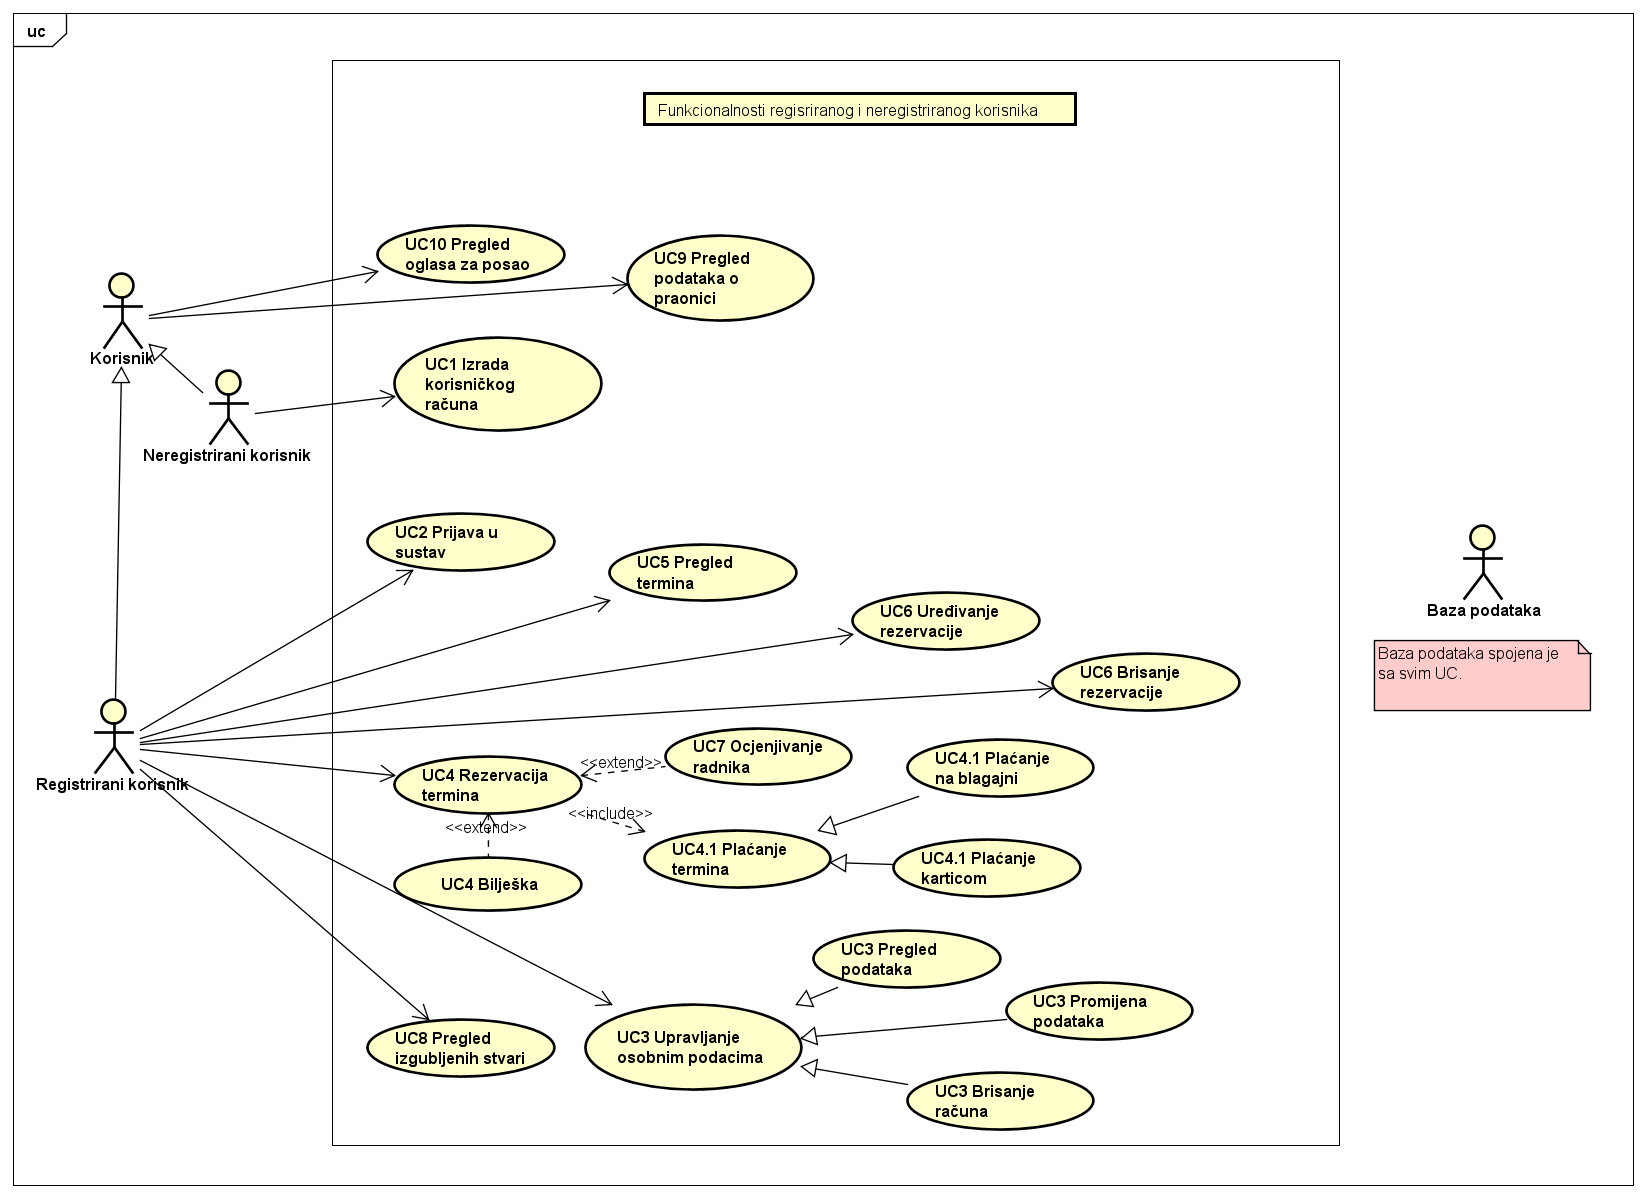
\includegraphics[width=.9\linewidth]{slike/DOU1.PNG}
	\caption{Slika dijagrama obrasca uporabe registriranih i neregistriranih korisnika}
	\label{fig:dou1}
\end{figure}

\subsection{Sekvencijski dijagrami}

\textbf{\textit{dio 1. revizije}}\\

\textit{Nacrtati sekvencijske dijagrame koji modeliraju najvažnije dijelove sustava (max. 4 dijagrama). Ukoliko postoji nedoumica oko odabira, razjasniti s asistentom. Uz svaki dijagram napisati detaljni opis dijagrama.}
\eject

\textbf{Obrazac uporabe UC1 i UC2 - Registracija i Prijava korisnika}\\

\textbf{TODO} napisati opise.


\begin{figure}[H]
	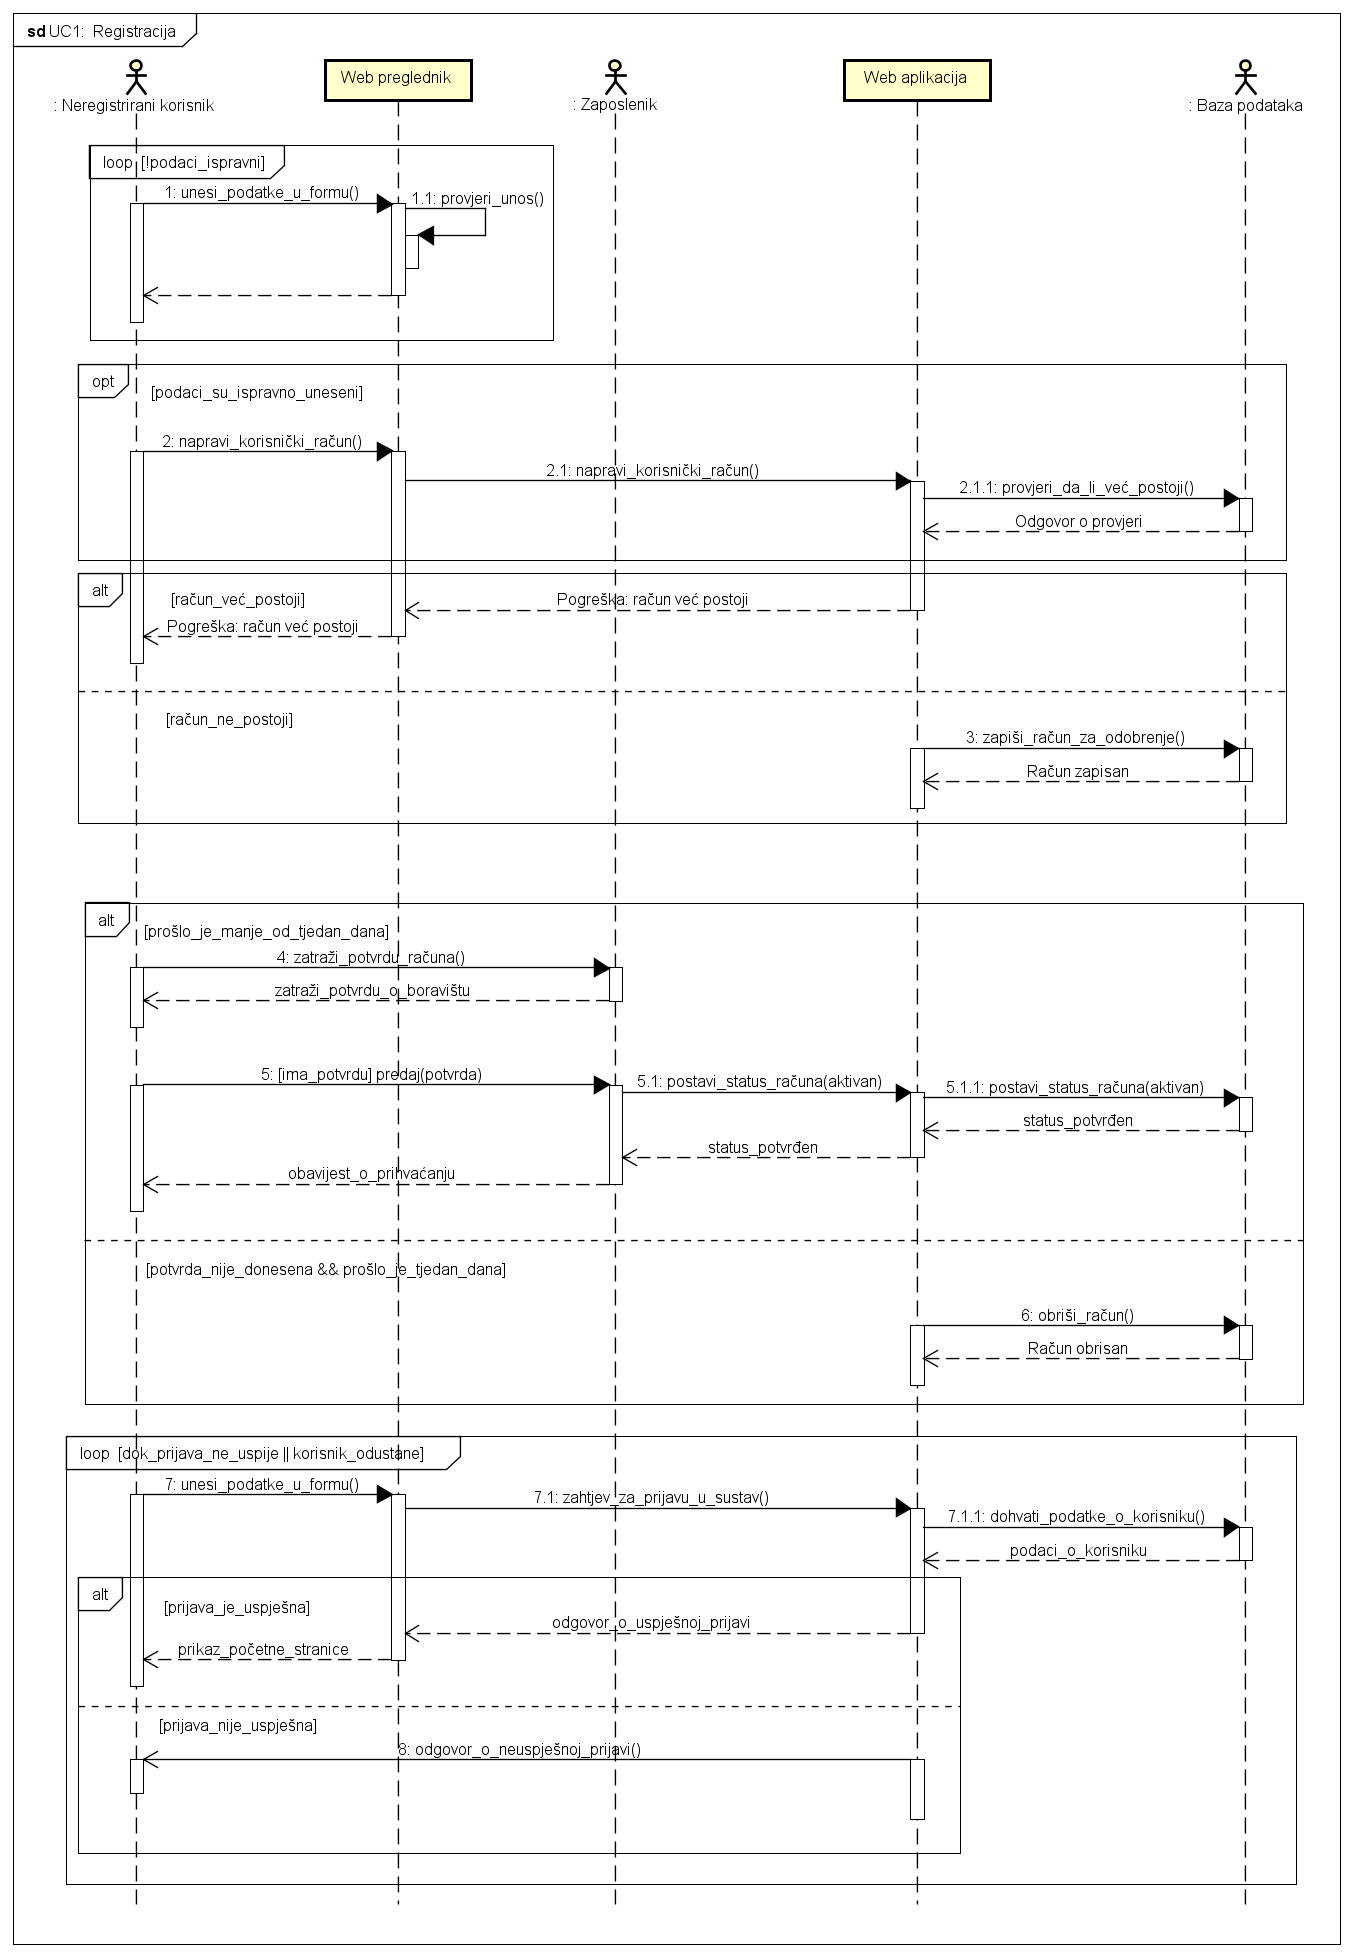
\includegraphics[width=.9\linewidth]{slike/UC1_Registracija.png}
	\caption{Sekvencijski dijagram za UC1 i UC2}
	\label{fig:skvDReg}
\end{figure}
\eject

\textbf{Obrazac uporabe UC3 - Pregled vlastitog profila i uređivanje podataka}\\

{Registrirani korisnik, zaposlenik ili admin odabire opciju za prikaz vlastitog profila. Web aplikacija dohvaća podatke o korisniku iz baze podataka te ih prikazuje na stranici profila. Korisnik može urediti svoje podatke. Klikom na gumb ya ismjenu podataka otvara se obrazac. Korisnik popunjava obrazac, a web aplikacija provjerava ispravnost popunjenih podataka. Ukoliko su podaci krivo popunjeni, web aplikacija ispisuje upozorenje, a promjena ostaje nezabilježena. Ispravno popunjen obrazac se pohranjuje u bazu podataka. }


\begin{figure}[H]
	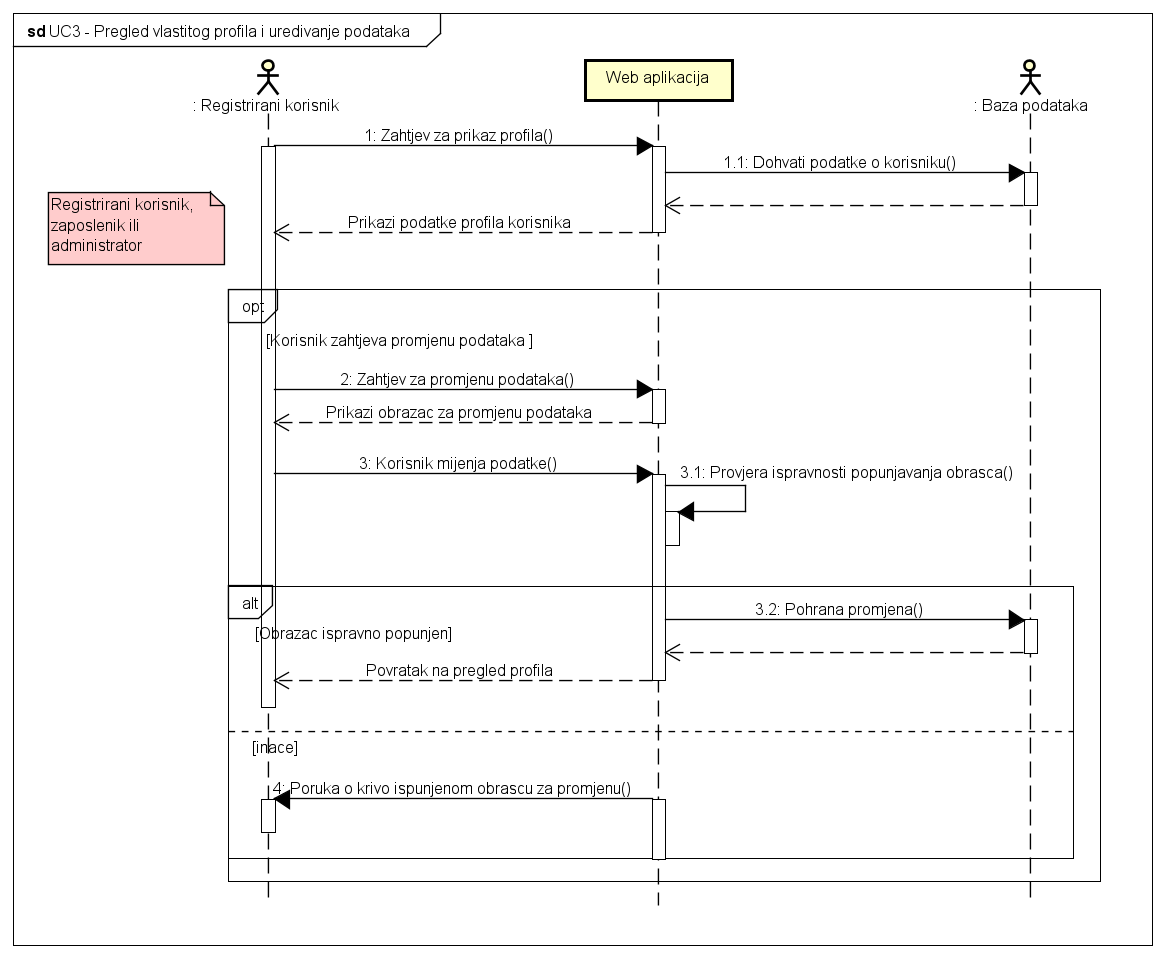
\includegraphics[scale=0.5]{slike/UC3_Pregled_vlastitog_profila.PNG} %veličina slike u odnosu na originalnu datoteku i pozicija slike
	\centering
	\caption{Sekvencijski dijagram za UC3}
	\label{fig:promjene}
\end{figure}

\textbf{Obrazac uporabe UC4 - Rezervacija termina za pranje veša}\\

{Registrirani korisnik odabire opciju za rezervaciju termina. Poslužitelj dohvaća podatke o terminima iz baze podataka i prikazuje kalendar sa slobodnim terminima registriranom korisniku. Korisnik odabire jedan od slobodnih termina, način plaćanja (online ili uživo) te može ostaviti bilješku. Podaci o terminu se pohranjuju u bazu podataka. Korisnik dobiva potvrdu o uspješnoj rezervaciji termina. Ukoliko nema slobodnih termina, korisniku se ispisuje poruka "Nema slobodnih termina".}


\begin{figure}[H]
	\includegraphics[scale=0.5]{slike/UC4_ Rezervacija_termina_za_pranje_veša.PNG} %veličina slike u odnosu na originalnu datoteku i pozicija slike
	\centering
	\caption{Sekvencijski dijagram za UC4}
	\label{fig:promjene}
\end{figure}


\textbf{Obrazac uporabe UC11 - Objava oglasa za posao} \\

\textbf{TODO} napisati opise.


\begin{figure}[H]
	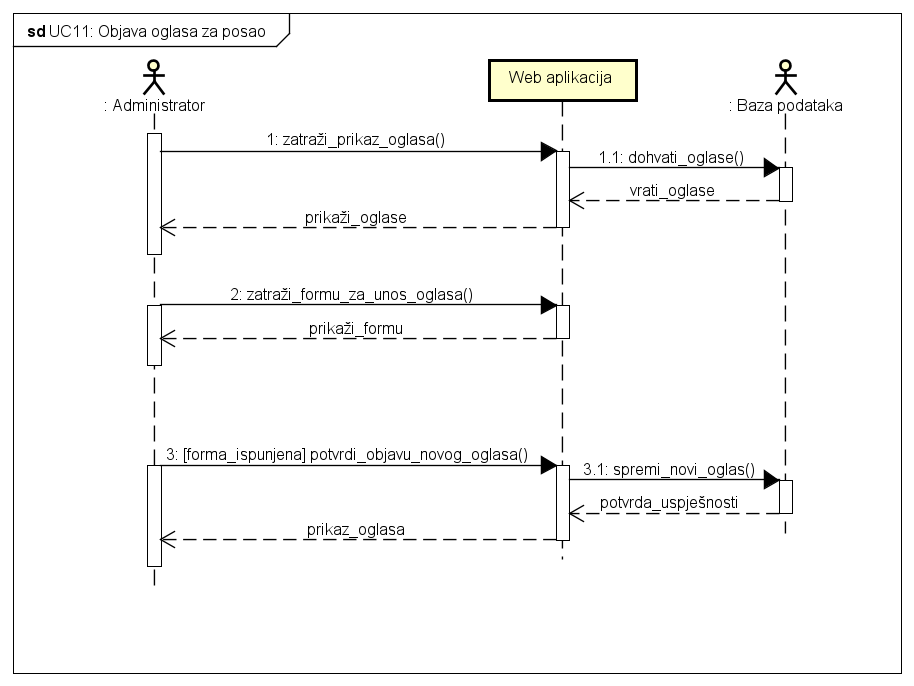
\includegraphics[width=.9\linewidth]{slike/UC11_Objava_oglasa_za_posao.png}
	\caption{Sekvencijski dijagram za UC11}
	\label{fig:skvDOglas}
\end{figure}
\eject

\section{Ostali zahtjevi}

\textbf{\textit{dio 1. revizije}}\\

\textit{Nefunkcionalni zahtjevi i zahtjevi domene primjene dopunjuju funkcionalne zahtjeve. Oni opisuju \textbf{kako se sustav treba ponašati} i koja \textbf{ograničenja} treba poštivati (performanse, korisničko iskustvo, pouzdanost, standardi kvalitete, sigurnost...). Primjeri takvih zahtjeva u Vašem projektu mogu biti: podržani jezici korisničkog sučelja, vrijeme odziva, najveći mogući podržani broj korisnika, podržane web/mobilne platforme, razina zaštite (protokoli komunikacije, kriptiranje...)... Svaki takav zahtjev potrebno je navesti u jednoj ili dvije rečenice.}

\begin{packed_item}
	\item Treba biti omogućen rad više korisnika u stvarnom vremenu
	\item Sustav i korisničko sučelje moraju imati podršku za sve znakove hrvatske abecede
	\item Dizajn korisničkog sučelja treba biti responzivan, odnosno takav da se može koristiti na svakom uređaju bez obzira na veličinu ekrana
	\item Potrebno je omogućiti korisniku zamjenu ili uređenje odabranog termina 24 sata prije početka
	\item Sustav će periodički svakih tjedan dana brisati nepotvrđene rezervacije iz baze podataka
	\item Radno vrijeme moći će se mijenjati za sve dane koji su dva tjedna nakon tekućeg dana
	\item Morati će postojati ograničenje rezervacije dva termina dnevno za svakog registriranog korisnika
	\item Neispravno korištenje korisničkog sučelja mora dati povratnu informaciju korisniku u stvarnom vremenu
	\item Sustav treba omogućiti korištenje kolačića (engl. \textit{cookies}) u svrhu pohrane privremeno korištenih podatka
	\item Sve novčane transakcije koristi HRK kao valutu
	\item Sustav treba biti dovoljno jednostavan kako bi ga mogla koristiti osoba bez opširnih uputa
	\item Lozinke korisnika u bazi podatka trebaju biti zaštićene PBKDF2 \textit{(Password-Based Key Derivation Function 2)}
kriptografskim algoritmom kako bi se smanjila mogućnost narušavanja sigurnosti sustava
	\item Pristup sustavu omogućen je korištenjem protokola HTTP/2
	
\end{packed_item}


